\section{実験}
\subsection{共通設定}
評価にはCOCO 2017 Validationを用いた．
前稿\cite{ref_prev}と同じく，seed 42で選んだ500枚を検証用，別の500枚をテスト用とした．
テスト用の画像のGTの物体は3458件（人物1090件，人物以外2368件）である．
閾値などの条件は全て検証用の画像で選び，テスト用の画像の結果を報告する．
COCO外の物体の評価には，テスト用の画像のうちLVIS v1\cite{ref_LVIS}の注釈がある474枚を用い，Synsetが COCOのクラスのSynsetの上位語，下位語，自身のいずれでもない2687件をCOCO外の物体とした．
VGの語彙にはVG v1.2の108077枚の物体の注釈を用い，COCO 2017 Validationと重複する2186枚を集計から除いた．
式(\ref{eq_vocab})の語彙は3263語（COCOの80クラスを加えて3293語），木は枠を含めて3315ノードである．
最上位の枠は前稿に一覧が無いため，clothing，furniture，animal，light，natural objectなどの40個を定めた．

検出器には，OWLv2（ViT-B/16，ensemble）\cite{ref_OWLv2}の物体らしさ（$ B = 20, 50 $），YOLO11x\cite{ref_YOLO11}（検出スコア0.25以上），DETR（ResNet-50，検出スコア0.5以上）\cite{ref_DETR}を用いた．
分類器には，Alpha-CLIP（ViT-B/16）\cite{ref_AlphaCLIP}とCLIP（ViT-B/32）\cite{ref_CLIP}を用いた．
参照として，前稿の構成（以下，Old）であるDETRのボックスの切り抜き画像にCLIPを適用し，COCOの80クラスの最大の確信度でボックスを残すものと，COCOで学習したYOLO11xが出力するクラスをそのまま用いるもの（以下，YOLO11x単体）を評価した．
YOLO11x単体以外は，いずれもCOCOのクラスの注釈を命名に用いない．
GPUにはNVIDIA GeForce RTX 4070 Tiを用い，いずれのモデルも再学習は行わない．

\begin{table}[t]
\centering
\caption{本稿の表で用いる記号と評価指標．}
\label{tab_metrics}
\setlength{\tabcolsep}{3pt}
\begin{tabular}{lp{0.68\linewidth}}
\toprule
記号 & 説明 \\
\midrule
$ B $ & OWLv2の1枚あたりの平均ボックス数（閾値を検証用の画像で決める） \\
$ N $ & 1枚あたりのボックス数（式(\ref{eq_score})の規則の後は残した数） \\
$ R_{\rm all} $ & 検出の再現率：クラスを問わずIoU 0.5以上のボックスがあるGTの割合 \\
$ R_{\rm per} $，$ R_{\rm oth} $ & $ R_{\rm all} $の人物のGT，人物以外のGTに限った値 \\
$ R_{\rm N} $ & COCO外の物体の再現率：LVISのCOCO外の物体を囲んだ割合 \\
$ E $ & どのGTともIoU 0.5以上で重ならないボックスの割合 \\
$ t $ & 1枚あたりの検出の時間（秒） \\
Top-1 & 対応したボックスのうち，ラベルがGTのクラスと一致した割合 \\
$ P $，$ R $，$ F $ & 適合率，再現率，F値：ラベルも一致した組を正解とする（COCOの80クラス） \\
$ hP $，$ hR $，$ hF $ & 細かい正解に対する階層的適合率，階層的再現率，階層的F値（式(\ref{eq_hier})） \\
$ \tau $，$ T $ & 出力の深さを決める確率の閾値と温度（式(\ref{eq_output})） \\
$ R_{\rm p} $ & 人物の再現率：人物のGTのうち，対応したボックスを残した割合 \\
Acc & 命名の正解率：細かい正解と一致，それより細かい，または正しい上位語を出力した割合 \\
Fine & 正しくCOCOのクラスより細かい語を出力した割合 \\
\bottomrule
\end{tabular}
\end{table}

評価指標を表\ref{tab_metrics}に示す．
COCOの80クラスによる指標では，スコアの降順に，IoUが0.5以上のGTと1対1に対応付け，Top-1，$ P $，$ R $，$ F $を求めた．
細かい粒度の指標では，COCOのキャプションの名詞をspaCyで取り出してWordNetの第1語義に変換し，GTのクラスのSynsetの真の下位語になる語を，その画像の同じクラスのインスタンスの細かい正解とした（例：person→man，woman，tennis player）．
細かい正解を持つインスタンスはテスト用の画像で912件であり，85\%が人物である．
前稿\cite{ref_prevVG}と同じく，出力$ u $と細かい正解$ g $について，Synset自身と深さ4以上の上位語の集合$ {\mathbb P}_k $，$ {\mathbb G}_k $を求め，

\begin{equation}
    hP = \frac{\sum_k |{\mathbb P}_k \cap {\mathbb G}_k|}{\sum_k |{\mathbb P}_k|}, \quad hR = \frac{\sum_k |{\mathbb P}_k \cap {\mathbb G}_k|}{\sum_k |{\mathbb G}_k|}
    \label{eq_hier}
\end{equation}

\noindent
とし，その調和平均を$ hF $とした．
ただし，person.n.01の深さは3であるため，COCOの80クラスのSynsetは深さによらず集合に含めた．
未検出または残さなかったインスタンスは$ {\mathbb P}_k = \emptyset $とする．
差の検定には，画像単位の対応のあるブートストラップ（1000回）を用いた．
式(\ref{eq_score})の$ \theta $は検証用の画像の$ F $で，式(\ref{eq_output})の$ T $と$ \tau $は検証用の画像の$ hF $で選んだ（Alpha-CLIPは$ T = 1 $，$ \tau = 0.05 $，CLIPは$ T = 1.5 $，$ \tau = 0.1 $）．

\subsection{検出器の比較}
\begin{table}[t]
\centering
\caption{検出器のみの比較（テスト用の画像）．$ R_{\rm N} $はLVISの注釈がある474枚のCOCO外の物体2687件に対する値，その他はCOCOのGT 3458件に対する値である．記号は表\ref{tab_metrics}による（$ N $：ボックス数，$ R_{\rm all} $：再現率，$ R_{\rm per} $：人物の再現率，$ R_{\rm oth} $：人物以外の再現率，$ E $：GTに当たらない割合，$ R_{\rm N} $：COCO外の物体の再現率，$ t $：時間）．}
\label{tab_detector}
\setlength{\tabcolsep}{2.5pt}
\resizebox{\linewidth}{!}{%
\begin{tabular}{lrrrrrrr}
\toprule
検出器 & $ N $ & $ R_{\rm all} $ & $ R_{\rm per} $ & $ R_{\rm oth} $ & $ E $ & $ R_{\rm N} $ & $ t $ \\
\midrule
YOLO11x & 6.2 & 0.702 & 0.800 & 0.657 & {\bf 0.201} & 0.100 & {\bf 0.016} \\
DETR & 11.2 & 0.738 & 0.828 & 0.697 & 0.475 & 0.124 & 0.049 \\
OWLv2（$ B = 20 $） & 18.4 & 0.700 & 0.541 & 0.774 & 0.739 & 0.519 & 0.232 \\
OWLv2（$ B = 50 $） & 46.6 & {\bf 0.875} & {\bf 0.883} & {\bf 0.871} & 0.867 & {\bf 0.734} & 0.232 \\
\bottomrule
\end{tabular}}
\end{table}

表\ref{tab_detector}に，検出器のみの比較を示す．
COCOの物体の再現率$ R_{\rm all} $は，OWLv2の$ B = 50 $が0.875で最も高く，DETRの0.738，YOLO11xの0.702を上回った．
ただし，OWLv2はボックスの数がYOLO11xの約7.5倍であり，GTに当たらないボックスの割合$ E $は0.867である．
$ B = 20 $では，$ R_{\rm all} $はYOLO11xと同程度であるが，人物の再現率$ R_{\rm per} $は0.541にとどまった．
密集した人物のボックスの物体らしさが低いためである．
COCO外の物体の再現率$ R_{\rm N} $は，OWLv2の$ B = 50 $が0.734，$ B = 20 $が0.519であるのに対し，YOLO11xは0.100，DETRは0.124であった．
COCOで学習した検出器は，COCO外の物体の領域をほとんど出力しない．

\begin{figure*}[t]
\centering
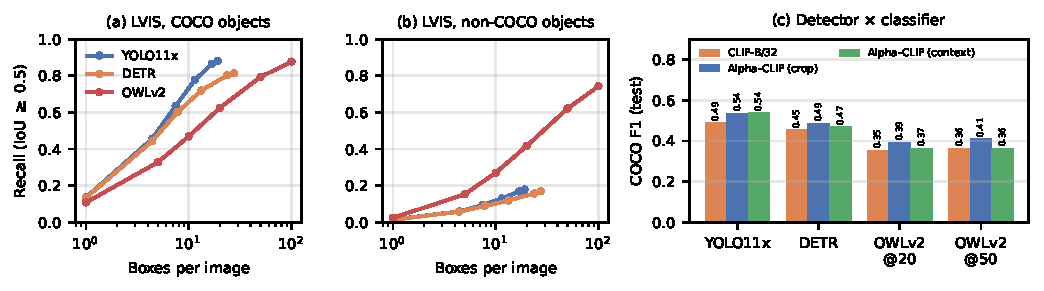
\includegraphics[width=\linewidth]{figures/fig_detector.pdf}
\caption{(a)(b) LVISの2148枚における1枚あたりのボックス数と検出の再現率（上位$ k $個のボックス，前稿の評価），(c) モデルの検出器と分類器を替えたテスト用の画像の$ F $（COCOの80クラスのF値）．}
\label{fig_detector}
\end{figure*}

図\ref{fig_detector}(a)(b)に，検出器の閾値を下げ，1枚あたり上位$ k $個のボックスを用いた場合の再現率を示す．
COCOの物体では，同じボックス数ならYOLO11xとDETRがOWLv2より高い．
YOLO11xとDETRは閾値を下げても約20〜30個でボックスが尽き，COCO外の物体の再現率は0.18以下にとどまった．
OWLv2は100個で0.743に達した．

\begin{table*}[t]
\vspace{4mm}
\centering
\caption{モデルの検出器を替えた比較（テスト用の画像，分類器はAlpha-CLIP（crop），残すボックスは式(\ref{eq_score})の規則）．記号は表\ref{tab_metrics}による（$ N $：残した数，Top-1：ラベルの正解率，$ P $：適合率，$ R $：再現率，$ F $：F値，$ hF $：細かい粒度の階層的F値，Acc：命名の正解率，Fine：正しくCOCOのクラスより細かい語を出力した割合，$ R_{\rm p} $：人物の再現率，$ R_{\rm N} $：残したボックスのCOCO外の物体の再現率）．}
\label{tab_pipeline}
\begin{tabular}{lrrrrrrrrrr}
\toprule
検出器 & $ N $ & Top-1 & $ P $ & $ R $ & $ F $ & $ hF $ & Acc & Fine & $ R_{\rm p} $ & $ R_{\rm N} $ \\
\midrule
YOLO11x（ボックスのみ） & 4.1 & 0.810 & {\bf 0.721} & 0.426 & {\bf 0.535} & 0.502 & 0.363 & 0.123 & 0.726 & 0.058 \\
DETR（ボックスのみ） & 5.3 & {\bf 0.819} & 0.562 & {\bf 0.428} & 0.486 & {\bf 0.521} & {\bf 0.385} & {\bf 0.136} & {\bf 0.739} & 0.061 \\
OWLv2（$ B = 20 $） & 4.4 & 0.777 & 0.507 & 0.322 & 0.394 & 0.428 & 0.235 & 0.104 & 0.421 & 0.094 \\
OWLv2（$ B = 50 $） & 5.3 & 0.796 & 0.472 & 0.363 & 0.411 & 0.461 & 0.274 & 0.111 & 0.545 & {\bf 0.103} \\
\midrule
Old（DETR＋CLIP） & 6.6 & 0.680 & 0.389 & 0.368 & 0.378 & 0.466 & 0.467 & 0.060 & 0.517 & -- \\
YOLO11x単体 & 5.7 & 0.976 & 0.796 & 0.655 & 0.719 & 0.670 & 0.816 & 0 & 0.766 & -- \\
\bottomrule
\end{tabular}
\end{table*}

表\ref{tab_pipeline}に，モデルの検出器を替えた検出から命名までの結果を示す．
$ F $はYOLO11xのボックスが0.535，DETRが0.486，OWLv2の$ B = 50 $が0.411であった．
OWLv2の$ B = 50 $との差は，YOLO11xが0.125（95\%区間［0.106，0.145］），DETRが0.075（［0.056，0.095］）であり，いずれも有意であった（$ p < 0.01 $）．
$ hF $もYOLO11xとDETRがOWLv2より0.04〜0.06高かった．
OWLv2の$ F $が低い主な原因は適合率$ P $であり，残したボックスのうちCOCOのGTに当たらないものが多い．
OWLv2の$ B = 50 $で残したボックスのうちCOCOのGTに当たらない41.3\%について，13.1\%はLVISのCOCO外の物体を囲んでいた（YOLO11xは7.0\%，DETRは3.4\%）．
LVISの注釈は網羅的でないため，この割合は下限である．
残したボックスのCOCO外の物体の再現率$ R_{\rm N} $は，OWLv2が0.103で最も高いものの，検出器の出力の0.734から大きく低下した．
$ \theta $をCOCOの80クラスの$ F $で選ぶため，COCO外の物体のボックスが残らないためである．
一方，COCOのクラスより細かい語を正しく出力した割合Fineは，いずれの検出器でも0.10〜0.14であり，Oldの0.060を上回った．
YOLO11x単体はCOCOの80クラスの$ F $が最も高いが，COCOのクラスより細かい語は出力できない．

\subsection{分類器の比較}
\begin{table}[t]
\centering
\caption{分類器の比較（テスト用の画像）．GTのボックスの列は検出の影響を除いた値であり，Top-1とTop-5はCOCOの80クラスの正解率，$ hF $は部分木の確率の合計による命名の階層的F値である（--：未評価）．右の4列は各検出器と組み合わせた場合の$ F $（COCOの80クラスのF値）である．}
\label{tab_classifier}
\setlength{\tabcolsep}{2.5pt}
\resizebox{\linewidth}{!}{%
\begin{tabular}{lrrrrrrr}
\toprule
 & \multicolumn{3}{c}{GTのボックス} & \multicolumn{4}{c}{$ F $（検出器と組み合わせ）} \\
分類器 & Top-1 & Top-5 & $ hF $ & YOLO & DETR & $ B {=} 20 $ & $ B {=} 50 $ \\
\midrule
CLIP（B/32） & 0.497 & 0.738 & 0.576 & 0.490 & 0.454 & 0.354 & 0.364 \\
Alpha-CLIP（crop） & {\bf 0.527} & 0.766 & -- & 0.535 & {\bf 0.486} & {\bf 0.394} & {\bf 0.411} \\
Alpha-CLIP（context） & {\bf 0.527} & {\bf 0.817} & {\bf 0.639} & {\bf 0.538} & 0.470 & 0.365 & 0.365 \\
\bottomrule
\end{tabular}}
\end{table}

表\ref{tab_classifier}に，分類器の比較を示す．
GTのボックスでは，Alpha-CLIPのTop-1は0.527であり，CLIPの0.497を上回った．
部分木の確率の合計による命名の$ hF $も，Alpha-CLIP（context）が0.639，CLIPが0.576であった（差0.063，［0.034，0.093］）．
検出器と組み合わせた場合，Alpha-CLIP（crop）の$ F $は，CLIPよりYOLO11xで0.045，DETRで0.032，OWLv2の$ B = 20 $で0.039，$ B = 50 $で0.047高く，いずれも有意であった（$ p \leq 0.001 $）．
Top-1も0.03〜0.07高かった．
一方，Alpha-CLIP（context）は，YOLO11xでは0.048高かったが，OWLv2ではCLIPとの差が有意でなかった．
contextの入力は周囲の領域を含むため，OWLv2の小さいボックスや物体の一部のボックスに周囲の物体の名前が付きやすい．
検出器と組み合わせた$ hF $の差は，いずれの組でも有意でなかった．
ただし，COCOのクラスより細かい語を正しく出力した割合Fineは，Alpha-CLIP（crop）が0.10〜0.14であり，CLIPの0.05〜0.06の約2倍であった．
命名の正解率AccはCLIPの方が0.12〜0.20高く，CLIPはpersonなどの粗い語を出力する割合が高い．
Alpha-CLIPは細かい語の確率を高く見積もるため，細かい語を出力する割合が増える一方，その一部は誤りとなる．
図\ref{fig_detector}(c)に，検出器と分類器の全ての組の$ F $を示す．

\subsection{語彙の木による粒度の判断}
本節では，検出の影響を除くため，GTのボックスに対して命名の手順を比較する．
VLMを用いない評価では，細かい正解のSynset自身がVGの語彙に含まれる割合は0.957であった．
語彙から1語を選ぶ場合の$ hR $の上限は，COCOの80クラスの0.597に対し，VGの語彙で0.990であった．

\begin{table}[t]
\centering
\caption{GTのボックスに対する命名の手順の比較（テスト用の画像）．$ hF $：細かい粒度の階層的F値，Acc：命名の正解率，Fine：正しくCOCOのクラスより細かい語を出力した割合．}
\label{tab_naming}
\setlength{\tabcolsep}{3pt}
\resizebox{\linewidth}{!}{%
\begin{tabular}{lrrrrrr}
\toprule
 & \multicolumn{3}{c}{CLIP（B/32）} & \multicolumn{3}{c}{Alpha-CLIP（context）} \\
命名の手順 & $ hF $ & Acc & Fine & $ hF $ & Acc & Fine \\
\midrule
COCOのクラスのみ & 0.373 & 0.518 & 0 & 0.266 & 0.307 & 0 \\
WordNetの下位語 & 0.373 & 0.503 & 0.029 & 0.266 & 0.304 & 0.015 \\
\rev{WordNet$ \cap $VGの木}の下位語 & 0.375 & 0.489 & 0.041 & 0.273 & 0.215 & 0.087 \\
VGの平坦な語彙 & 0.321 & 0.123 & 0.117 & 0.334 & 0.135 & 0.123 \\
部分木の合計 & 0.576 & 0.758 & 0.045 & {\bf 0.639} & {\bf 0.782} & 0.080 \\
\bottomrule
\end{tabular}}
\end{table}

表\ref{tab_naming}に結果を示す．
条件はいずれも検証用の画像の$ hF $で選んだ．
WordNetの下位語と\rev{WordNet$ \cap $VGの木}の下位語は，COCOのクラスから子のうち確率が最大の語を選んで下る手順である．
部分木の確率の合計は$ hF $を大きく高め，Alpha-CLIPではCOCOのクラスのみとWordNetの下位語の0.266から0.639に向上した．
VLMが人物の領域で持ち物の名前を最大にする場合でも，人物の部分木の確率が集まってpersonを出力できるためである．
部分木の確率の合計ではAlpha-CLIPがCLIPを上回ったのに対し，COCOのクラスのみでは下回った．
一方，COCOのクラスより細かい語を正しく出力できた割合は最大でも12.3\%であった．

\begin{figure}[t]
\centering
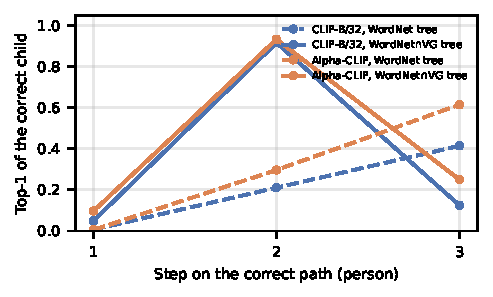
\includegraphics[width=0.95\linewidth]{figures/fig_step.pdf}
\caption{人物のGTのボックスで正しい経路を1段ずつ与えた場合の，各段の正しい子の選択の正解率（Top-1）．}
\label{fig_step}
\end{figure}

下位語をたどる手順が細かい語に届かない原因を調べるため，人物のGTのボックスで正しい経路を1段ずつ与え，各段で正しい子を選べる割合を求めた．
図\ref{fig_step}に結果を示す．
WordNetではpersonの直接の下位語が398語あり，1段目の正解率はAlpha-CLIPで0.005にとどまった．
\rev{WordNet$ \cap $VGの木}ではpersonの子が136語となり，1段目の正解率は0.097，2段目は0.933であった．

\subsection{定性評価}
図\ref{fig_qualitative}に，テスト用の画像に対する出力の例を示す．
(a)〜(c)では，部分木の確率の合計で選んだ語と，括弧内に深さ0のラベルを示す．
いずれの検出器でも，人物の領域にswimmer，surfer，tennis player，spectatorなどの細かい語が付き，同じ出力から深さ0のpersonも得られた．
YOLO11x単体はpersonのみを出力し，細かい語は出力できない．
OWLv2は波全体や画像全体などの大きな領域も囲み，surferのような場面の語を付けることがある．

\begin{figure*}[t]
\centering
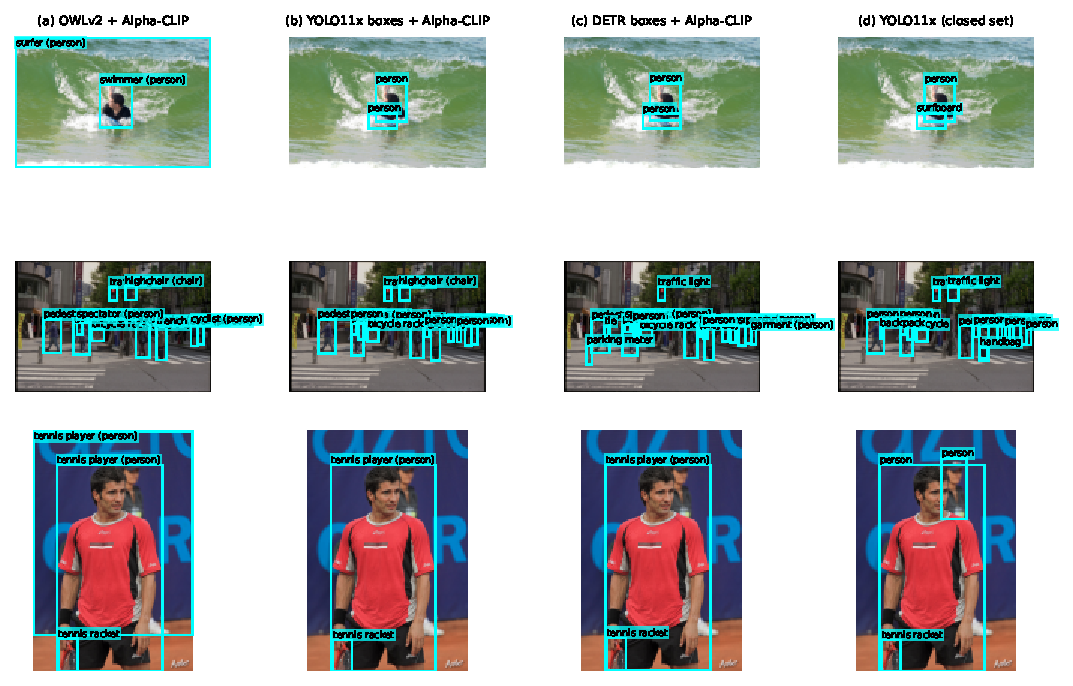
\includegraphics[width=0.82\linewidth]{figures/fig_qualitative.pdf}
\caption{テスト用の画像に対する出力の例．(a) OWLv2，(b) YOLO11xのボックス，(c) DETRのボックス（分類器はいずれもAlpha-CLIP（crop）），(d) YOLO11x単体．(a)〜(c)のラベルは式(\ref{eq_output})の出力であり，括弧内は深さ0のラベル$ c_k $である．}
\label{fig_qualitative}
\end{figure*}
